p\documentclass[a4paper, twoside]{article}

\usepackage[utf8]{inputenc}
\usepackage{listings}
\usepackage{tikz}
\usetikzlibrary{automata,positioning}
\usepackage{amsmath,amssymb,amsfonts}
\usepackage{todonotes}

\begin{document}

\title{Model Checking with Spin}
\author{Lukas Hofmaier \texttt{lukas.hofmaier@hsr.ch}}

\maketitle
\tableofcontents

\section{Model Checking}
\label{sec:modelchecking}

The Goal of a model checker is to verify behavioral models. That is, a model checker verifies whether a condition for a given model holds. Spin is a model checker. The model is described in Promela. Promela is a system specification language. The condition or property is described by linear temporal logic. In the next section model checking is compared to other verification methods. The section describes the advantages of model checking. The next next section explains how to use Promela to describe the behavior of a model. The next section describes correctness properties in general and how to define properties with temporal linear logic(LTL). Spin takes Promela source code and the LTL Properties as input and tells the user if the model holds for the defined properties.

\subsection{Why Model Checking}
\label{sec:why}

Among others, there are two options to verify software
\begin{description}
\item[Peer reviewing] Code is analyzed statically. Since the code is not compiled and executed, it is difficult to detect errors, caused by concurrency.
\item[Software testing] Software is compiled and executed. The system reads explicitly defined input and a subset of all possible paths is executed. The Output is compared with the specification. Practically, it is impossible to cover all possible paths through testing. Testing can expose errors. It doesn't proofs the absence of errors.
\end{description}

Peer reviewing and testing are both unable to verify 100\% of all possible cases. In a model-based verification a behavioral model is written and correctness properties are defined. A model checker processes the model and the properties and checks if the properties hold for the defined model. If the properties don't hold the model checker presents the user a counterexample. A counterexsample is a sequence of states which resulted in a undesirable state \cite{baier08}.

\section{Modeling Concurrent Systems}
\label{sec:concurrency}

This section shows how models are described in Promela and how concurrency affects the state diagram of a system. Mapping a real program to a Promela Model would be costly and time-expensive. Only the relevant or critical parts of the system are modeled and not every state of a program.


\subsection{Interleaving}
\label{sec:interleaving}

In this section programs are modeled as state diagrams. A state represents the program counter and the values of all variables in the program. The program counter points to the next statement. A transition represents the execution of the next statement and an increment of the program counter. Figure \ref{fig:sequencielstatediagram} shows a state diagram of a sequential program. 

\begin{figure}
 \centering
  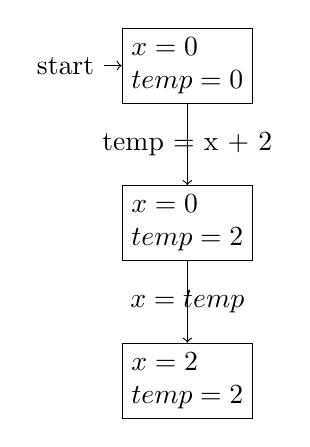
\begin{tikzpicture}[node distance=2cm, on grid, scale=0.5]
    \node[state, initial, rectangle, align=left](s1){$x=0$\\ $temp=0$};
    \node[state, rectangle, align=left, below =of s1](s2){$x=0$\\$temp=2$};
    \node[state, rectangle, align=left, below =of s2](s3){$x=2$\\$temp=2$};
    \path[->](s1) edge node {temp = x + 2}(s2);
    \path[->](s2) edge node {$x=temp$}(s3);
  \end{tikzpicture}

  \caption{State diagram of a system with a single process}
  \label{fig:sequencielstatediagram}
\end{figure}

In a sequential program with one process, there is one possibility in which order the statements are executed. Each state has only outgoing transition. When multiple processes are executed and the scheduler strategy is a priori unknown, there are several possibilities in which order the statements are executed. Interleaving is a paradigm to model systems with multiple processes. This perspective is based on the view that only one processor is available on which the statements of the programs are interlocked \cite{baier08}. In each state there is a nondeterministic choice, which process can execute the next statement. Figure \ref{fig:interleavingtransitionsystem} shows a state diagram of a system with two processes. Interleaving is a enumeration of all possible state sequences.

\subsection{Interleaving Examples}
\label{sec:interleavingexamples}

\subsubsection{Promela}
\label{sec:promela}

Spin verifies models of system behavior, written in the system specification language Promela. In the following section, concepts are explained by Promela code examples. This section is intended to contribute to the understanding of the code examples.

Promela is intended to describe abstractions of systems designs. It's specification language. A Promela model describes the behavior of a system. Promela is intended to to descripe concurrent software systems.

The syntax for declaration of variables is similiar to the programming language C. In the following examples use the data type byte.

A keyword is defined with the keyword \verb|proctype|. \verb|proctype| is followed by the identifier of the process. The statements of the process type is enclosed in curly braces \verb|{}| \cite{holzmann03}.

The keyword \verb|active| creates a new process instance of the following process type. The process starts immediately.

\subsubsection{Sequential Programming}
\label{sec:sequential}

Listing \ref{lst:interleavingcode} shows a system with one active process. The statements are executed sequentially. A instance of the process type \verb|sequential| is created. The process reads the global variable \verb|x|, computes $x+2$ and stores the result in the variable \verb|temp|. Then \verb|temp| is assigned \verb|x|. The order of the states of the corresponding state diagram is non-ambiguous. Figure \ref{fig:sequencielstatediagram} shows the state diagram.

 \lstinputlisting[float,label={lst:interleavingcode},caption={system with a single process},numbers={left},float,language=Promela]{sequential.pml}  

\subsubsection{Concurrent Programming}
\label{sec:concurrent}

Listing \ref{list:interleaving2proc} shows a system with 2 active processes. The processes are executed concurrently. The processes add a constant integer to the global variable \verb|x| like the system in section \ref{sec:sequential}. There are several possibilites the computation is executed. One possible computation would first execute all statements of process \verb|A| and then all statements of process \verb|B|. The scheduler can switch the process after every transition. Figure \ref{fig:interleavingtransitionsystem} shows the interleaved state diagram of the system in Listing \ref{list:interleaving2proc}.

\lstinputlisting[label=list:interleaving2proc, caption={Add operation with 2 processes},numbers=left,float,language=Promela]{interleavingproc.pml}  

\begin{figure}
\centering

 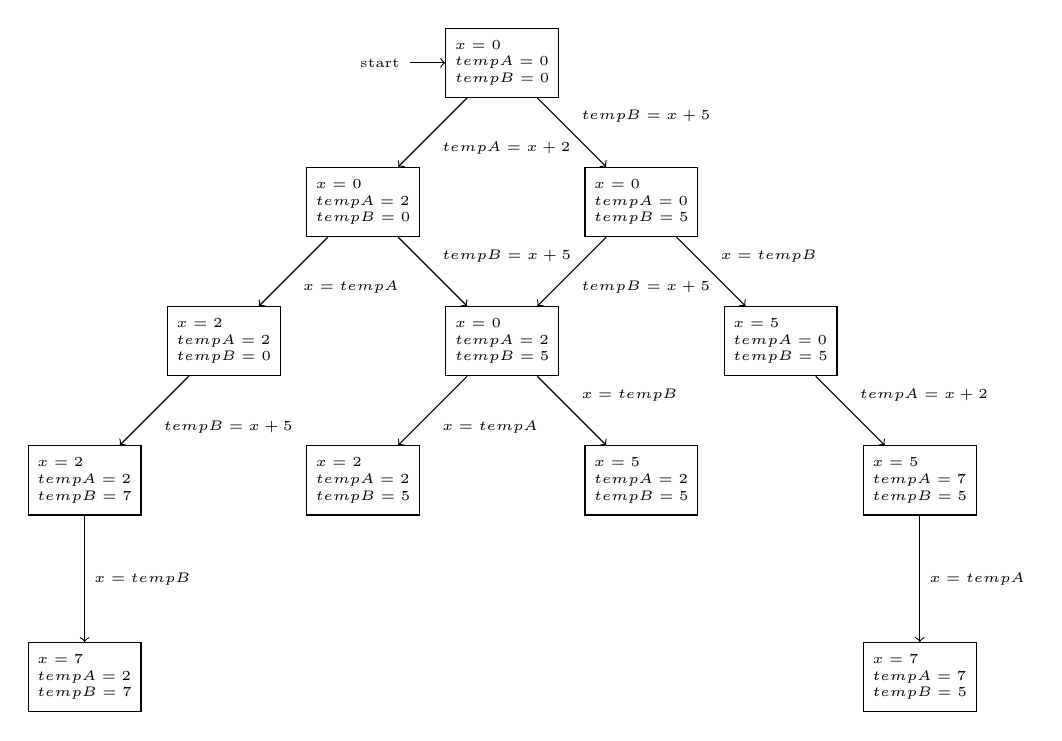
\begin{tikzpicture}[node distance=2.5cm, on grid, auto]
\tikzstyle{every node}=[font=\tiny]
   \node[state, initial, rectangle, align=left](s1){$x=0$\\$tempA=0$\\$tempB=0$};
   \node[state, rectangle, align=left](s2) [below left=of s1]{$x=0$\\$tempA=2$\\$tempB=0$};
   \node[state, rectangle, align=left](s3)[below left=of s2]{$x=2$\\$tempA=2$\\$tempB=0$};
  \node[state, rectangle, align=left](s4)[below left=of s3]{$x=2$\\$tempA=2$\\$tempB=7$};
\node[state, rectangle, align=left](s5)[below =of s4]{$x=7$\\$tempA=2$\\$tempB=7$};
\node[state, rectangle, align=left](s6)[below right=of s1]{$x=0$\\$tempA=0$\\$tempB=5$};
\node[state, rectangle, align=left](s7)[below right=of s6]{$x=5$\\$tempA=0$\\$tempB=5$};
\node[state, rectangle, align=left](s8)[below right=of s7]{$x=5$\\$tempA=7$\\$tempB=5$};
\node[state, rectangle, align=left](s9)[below =of s8]{$x=7$\\$tempA=7$\\$tempB=5$};
\node[state, rectangle, align=left](s10)[below right=of s2]{$x=0$\\$tempA=2$\\$tempB=5$};
\node[state, rectangle, align=left](s11)[below left=of s10]{$x=2$\\$tempA=2$\\$tempB=5$};
\node[state, rectangle, align=left](s12)[below right=of s10]{$x=5$\\$tempA=2$\\$tempB=5$};
   \path[->](s1) edge node {$tempA=x+2$}(s2);
   \path[->](s2) edge node {$x=tempA$}(s3);
   \path[->](s3) edge node {$tempB=x+5$}(s4);
\path[->](s4) edge node {$x=tempB$}(s5);
\path[->](s1) edge node {$tempB=x+5$}(s6);
\path[->](s6) edge node {$x=tempB$}(s7);
\path[->](s7) edge node {$tempA=x+2$}(s8);
\path[->](s8) edge node {$x=tempA$}(s9);
\path[->](s2) edge node {$tempB=x+5$}(s10);
\path[->](s6) edge node {$tempB=x+5$}(s10);
\path[->](s10) edge node {$x=tempA$}(s11);
\path[->](s10) edge node {$x=tempB$}(s12);

 \end{tikzpicture}   

 \caption{State diagram for system in Listing \ref{list:interleaving2proc}}
\label{fig:interleavingtransitionsystem}
 \end{figure}

The state diagram \ref{fig:interleavingtransitionsystem} shows that the system from Listing \ref{list:interleaving2proc} can terminate in 4 different states. If the scheduler strategy is unknow the resulting state is non-deterministic. Modelchecking tools like spin are able search the state space for unwanted states. Undesirable states are defined with Lineare Temporal Logic. Section \ref{sec:ltl} will explain how undesirable is defined.

\subsection{Synchronization}
\label{sec:synchronization}

\subsubsection{Synchronization Example}
\label{sec:syncexample}

Listing \ref{lst:withoutsemaphore} shows a system with two active processes with the same process type. The processes are instantiated within the \verb|init|-process. It is always the first process activated. Both processes add the value $2$ to the value stored in \verb|x|. If you like to enforce that the resulting value in \verb|x| is $4$, you have to synchronize the processes. Only one process can be in the critical section (line 4-8). This is also called mutual exclusion. One way to achieve mutual exclusion is the use of semaphores.

Listing \ref{lst:withsemaphore} shows a system that achieves mutual exclusion with semaphores. When this system terminates, the variable \verb|x| has always the value $4$.

\lstinputlisting[label={lst:withoutsemaphore},caption={Program without mutual exlusion}, numbers=left,float,language=Promela]{withoutsemaphore.pml}

The Test \verb|x>0| and the following \verb|x--|-Operation have to be executed atomic. In Promela atomic sequences of statements are enclosed in curly braces with a preceding \verb|atomic| keyword.

Boolean expression like \verb|x>0|, without an assignment block processes when the expression evaluates to False until it evaluates to True.

\lstinputlisting[label={lst:withsemaphore},numbers=left,float,language=Promela,caption={Mutual exlusion with semaphores}]{semaphore.pml}

\subsubsection{Deadlock Example}
\label{sec:deadlock}

When system contains more than one lock, a deadlock may occur. Listing \ref{list:deadlock} shows a system that contains a deadlock. Given the sequence process \verb|TakeAFirst| requests semaphore $A$ and in the next executed state process $B$ requests semaphore $B$. Both processes are waiting for the other semaphore to proceed. The system is dead.

Section \ref{sec:ltl} describes how spin can detect deadlock in systems specified with Promela.

\lstinputlisting[label=list:deadlock,numbers=left,float,language=Promela,caption={Synchronization with deadlock}]{deadlock.pml}

\section{Correctness Properties}
\label{sec:ltl}

The goal of model checking is to verify a behavioral model of the system against desired properties. This properties are called correctness properties. Examples for correctness properties are mutual exclusion and deadlock freedom. 

Spin read correctness properties in a formal Form, called Linear Temporal Logic(LTL). This section explains correctness properties and LTL. For a better understanding of correctness properties atomic propositions and traces are described first. Atomic propositions are part of an LTL-Formula. And Traces are important because correctness properties verify traces.

\subsection{Atomic Propositions}
\label{sec:atomicpropositions}

Atomic propositions are typse of declarative sentences which can either true or false. They evaluate to \verb|True| or \verb|False|. The evaluation depends on the state the system is in. The expression \verb|crit < 2| is a atomic proposition. Atomic propositions can be replaced by identifiers. For exmaple, it is possible to define the sentence ``Process \verb|TakeAFirst| has aquired \verb|mutexA| and waits for \verb|mutexB| to be released.'' as $waitA$  that references the system in listing \ref{list:deadlock}. This example is used in section \ref{sec:safety} to describe deadlock freedom.
 
We define $AP$ as a set of atomic propositions of a system to be verified. We can map to every state a set of atomic propositions who evaluate to \verb|True|. That set of each state is subset of $2^{AP}$.

Atomic propositions can be combined with propositional logic's operators (see table \ref{tab:operators_of_propositionallogic}.

\begin{table}
  \centering

  \begin{tabular}{l l l}
    Operator & Math & Spin \\
    not & $\neg$ & \verb|!| \\
    and & $\land$ & \verb|&&| \\
  \end{tabular}
  \caption{Operators of propositional logic }
  \label{tab:operators_of_propositionallogic}
\end{table}

\subsection{Traces}
\label{sec:traces}

The models that describe the behavior of a system in section \ref{sec:interleaving} can be executed in a simulation. The execution is one possible computation, a sequence of states. If the computation terminates as desired (in reactive system, computation typically do not terminate) a possible sequence starts in a initial state and ends in a defined terminal state. Every state can be mapped to a subset of $2^{AP}$. This subset contains atomic proposition that evaluate to \verb|True| in this state. A trace is a sequence of this subsets. Hence, a trace is a word over the alphabet $2^{AP}$.

A system $S$ can have multiple sequences of states. Hence, there are multiple traces in $S$. All traces of a system $S$ are referred as $Traces(S)$. $Traces(S)$ defines a language.

\subsubsection{Traceexample}
\label{sec:traceexample}

In this section presents an example trace. The system, that could produce the trace is shown in listing \ref{lst:criticalsection}.

\lstinputlisting[label=lst:criticalsection,caption={Critical section problem},numbers=left]{criticalsection.pml}

For a better understanding, the sequence of states is first show. A state can be represented as a triple, containing the value of the variable \verb|crit| and the locations counters of process \verb|A| and process \verb|B|. The first value shows the line number of the location counter of process \verb|A| and the second the line number of process \verb|B|.

A possible sequence $\pi$ of states, would be:

\begin{equation}
  \label{eq:path}
  \begin{split}
\pi = (4, 9, {critA}={False},{critB}=False) \rightarrow \\
(6, 9, {critA}={True},{critB}=False) \rightarrow \\
(7, 9, {critA}={False},{critB}=False) \rightarrow \\
(7, 11, {critA}={False},{critB}=True) \rightarrow \\
(7, 12, {critA}={False},{critB}=False)
  \end{split}
\end{equation}

In this example the two Boolean variables \verb|critA| and \verb|critB| are the atomic propositions. The set of all atomic propositions in the system is

\[
\text{AP}=\{critA, critB\}
\].

The trace to the sequence of states show in equation \ref{eq:path} produces the word

\[
trace(\pi) = \varnothing \{critA\} \varnothing \{critB\} \varnothing
\].

\subsection{Linear-Time Properties}
\label{sec:satisfactionrelations}

Linear-time Properties legen fest welche W"orter von einem System akzeptiert werden d"urfen. Ein Linear-time property ist eine Sprache "uber dem Alphabet $2^{AP}$.
Wenn $P$ ein LT Property und $S$ das modellierte System ist, dann erf"ullt $S$ $P$ (man schreibt $S \models P$) wenn Traces(S) $ Traces(S) \subseteq P $

\[
TS \models P \iff Traces(S) \subseteq P 
\]

$ \models $ ist eine satisfaction relation. 

Linear-time Properties k"onnen in Safety-, Liveness- und Fairness-Properties unterteilt werden. In den Abschnitten \ref{sec:safety} und \ref{sec:liveness} werden Safety- und Liveness-Properties erkl"art.

\subsubsection{Safety-properties}
\label{sec:safety}

Ein Safety-Property verifiziert, ob ein System unerw"unschte states enth"alt. 

Deadlock ist ein safety property. Deadlockfreiheit im System aus Listing \ref{list:deadlock} kann wie folgt als safety property definiert werden. Die atomic propositions $waitA$ und $waitB$ bezeichnen die Zust"ande, dass die processes \verb|TakeBFirst| und \verb|TakeAFirst| jeweils auf die anderen Mutex warten. Dann muss die Aussagenlogikformel  $\phi=\neg waitA \lor \neg waitB$ in jedem state True sein. Formell:

\[
P_{dlock} = {A_0 A_1 A_2 \dots \in (2^{AP})^{\omega} | \forall \geq i.   A_i \models \phi}
\]

wobei $(2^{AP})^{\omega}$ die Menge aller m"oglichen W"orter "uber $2^{AP}$ ist.

Auch Mutual exlusion kann mit einem Safety-Property verifiziert werden. Ein Safety-Property $P_{mutex}$ um mutual exlusion im System aus Listing \ref{lst:criticalsection} sicherzustellen, definiert eine Sprache in der keine W"orter mit $\{critA,critB\}$ vorkommen d"urfen. Formell:
\[
P_{mutex} = \text{Menge aller W"orter} A_0 A_1 A_2 \dots \text{mit } \{critA,critB\} \not \subseteq A_i \text{ f"ur alle } 0 \leq i
\]
\[
 = {A_0 A_1 A_2 \dots \in (2^{AP})^{\omega} | \forall \geq i.   A_i \models \neg critA \lor \neg critB}
\]

Ein Modelchecker "uberpr"uft, ob Traces(S) eines Systems $S$ ein Wort (trace) enth"alt, dass die Anforderung des definierten Property nicht erf"ullt.

\subsubsection{Liveness-Properties}
\label{sec:liveness}

Safety-Properties definieren, dass in einer Sprache bestimmte Prefixe nicht vorkommen. Ein System $S$ das nichts tun w"urde, dass heisst $Traces(S)=\varnothing$ w"urde jedes Safety-Property erf"ullen. Fortschritt muss auch verfiziert werden k"onnen. Liveness-Properties definieren, dass jeder Trace in einem System erweitert werden kann, sodass das resultierende Wort das Liveness-Property erf"ullt.

Ein Liveness-Property fordert, dass sich gewisse events unendlich oft wiederholen. Liveness-Properties k"onnen nur von einem infiniten Trace erf"ullt werden. 

Starvation freedom ist ein Liveness Property. Starvation freedom fordert, dass jeder wartende Process eventuell seine critical section betritt. In einem infiniten Trace gibt es kein Prefix, dass starvation freedom verletzt. Aufgrund eines Prefix in einem infinten Trace kann man nicht "uberpr"ufen, ob ein Sachverhalt in Zukunft eintreten wird.

Formell kann man starvation freedom folgendermassen ausdr"ucken.
\[
P_{Starv} = \text{Menge aller infiniten W"orter } A_0 A_1 \dots A_j \in AP \text{ so dass }\exists j \geq 0. critA \in A_j
\]
\[
 = { A_0 A_1 \dots A_j \in (2^{AP})^{\omega} \exists j \geq 0. critA \in A_j}
\]

Listing \ref{lst:starvation} zeigt ein System $S_{Spinlock}$ bei dem starvation freedom nicht erf"ullt ist. Process A versucht den \verb|mutexB| mit einem Spinlock zu erlangen. In diesem System gibt es Traces, bei denen Process A in einem unendliche Loop versucht \verb|mutexB| zu erlangen und so nie in die eigene critical section kommt. Ein solcher Trace erf"ullt das LTL-Property \verb|<>critA| nicht. $S_{Spinlock}$ erf"ullt $P_{Starv}$ nicht.

\lstinputlisting[label={lst:starvation},caption={Critical section with starvation},numbers=left, language=Promela,float]{starvation.pml}

\subsection{Linear Temporal Logic}
\label{sec:lineartemporallogic}

M"ochte man ein Model, dass in Promela definiert ist, von Spin verifizieren lassen, muss man Spin das Model als Promela Source Code und die Definition eines Correctness-Property geben. Die Safety und Liveness-Properties aus Abschnitt \ref{sec:safety} und \ref{sec:liveness} sind ungeeignet f"ur die Eingabe. Linear Temporal Logic ist ein Formalismus mit dem Correctness Properties einfacher formuliert werden k"onnen.

Ein LTL-Formel besteht aus atomic propositions, die mit Operatoren der Aussagenlogik  und der temporal logic verkn"upft werden.

Mit atomic propositions kann man nur "uberpr"ufen, ob ein property in einem gegebenen state $s$ wahr oder falsch ist. M"ochte man beispielsweise mutual exlusion in Program \ref{lst:withoutsemaphore} ausdr"ucken, ben"otigt man Operatoren, die sich auf alle m"oglichen states beziehen. Temporal operators erm"oglichen solche Aussagen (siehe Tabelle \ref{tab:temporal_operators}). Die Formel k"onnen mit ASCI-Character ausgedr"uckt werden. Diese Form eignet sich f"ur die Eingabe von Spin.

\begin{table}
  \centering
  \begin{tabular}{l l l}
    Operator & Math & Spin \\
    always & $\square$ & \verb|[]| \\
    eventually & $\lozenge$ & \verb|<>| \\
    implies & $\implies$ & \verb|->| \\
    until & $U$ & \verb|U|
  \end{tabular}
  \caption{Temporal operators }
  \label{tab:temporal_operators}
\end{table}

Das Mutual Exlusion Safetyproperty $P_{mutex}$ aus Abschnitt \ref{sec:safety} kann in LTL pr"agnanter definiert werden
\[
  {A_0 A_1 A_2 \dots \in (2^{AP})^{\omega} | \forall \geq i.   A_i \models \neg critA \lor \neg critB}
\]

\[
= \square \neg (critA,critB)
\]

Das Livenessproperty $P_{Starv}$ f"ur Starvation freedom wird in LTL wie folgt definiert:
\[
 { A_0 A_1 \dots A_j \in (2^{AP})^{\omega} \exists j \geq 0. critA \in A_j}
\]

\[
= \lozenge critA
\]

\section{Example: Traffic light system}
\label{sec:example}

This section presents an example model in Promela and verification with LTL. The example is taken from \cite{kleuker09}. In this example a simple traffic light system for a crossroads is modeled. A Traffic light have two states: green and red. The model contains only 2 instead of 4 traffic lights because opposed traffic light have always the same state. The two traffic lights are numbered with 1 and 2.

\subsection{Requirements}
\label{sec:requirements}

The following requirements are demanded
\begin{enumerate}
\item the traffic lights are either red or green
\item The traffic light switch repetitive between red and green.
\item Only one traffic light is green at a time.
\item The traffic light turn alternating to green.
\end{enumerate}

\subsection{Atomic propositions}
\label{sec:trafficlightap}

First the atomic propositions for the LTL-Formulas are defined:

\begin{description}
\item[tl1green] Traffic light 1 is green.
\item[tl1red] Traffic light 1 is red.
\item[tl2green] Traffic light 2 is green.
\item[tl2red] Traffic light 2 is red.
\item[tl1last] Traffic light 1 was green last.
\item[tl2last] Traffic light 2 was green last.
\end{description}

\subsection{LTL-Formulas}
\label{sec:exampleltl}

The requirements can be formalized as follows:

\begin{enumerate}
\item 
  \begin{multline}
    (((\text{tl1green} \lor \text{tl1red}) \land (\text{tl1green}\iff \neg \text{tl1red})) \\ \land((\text{tl2green} \lor \text{tl2red})\land (\text{tl2green} \iff \neg \text{tl2red})))
  \end{multline}
\item
  \begin{multline}
    \label{eq:unnumbered}
    (((\text{tl1green} \implies (\lozenge \text{tl1red})) \\
    \land (\text{tlred} \implies (\lozenge \text{tl1green}))\\
    \land (\text{tl2green} \implies (\lozenge \text{tl2red})) \\
    \land (\text{tl2red} \implies (\lozenge \text{tl2green}))))
  \end{multline}
\item
  \begin{multline}
    \label{eq:unnumbered}
    ((\text{tl1green} \implies \neg \text{tl2green}) \land (\text{tl2green} \implies \neg \text{tl1green}))
  \end{multline}
\item
  \begin{multline}
    \label{eq:unnumbered}
    ((\text{tl1last} U(\text{tl2last} \land \neg \text{tl1last})) \\
    \land (\text{tl2last} U (\text{tl1last} \land \neg \text{tl2last}))\\
\land(\text{tl1zuletzt} \iff \neg \text{tl2last}))
  \end{multline}

\subsection{Promela Model}
\label{sec:trafficlightsmodel}

\lstinputlisting[label={lst:trafficlightsmodel},caption={Promelamodel of the traffic light system}n,umbers=left,language=Promela,float]{trafficlights.pml}

\end{enumerate}


\appendix

\begin{thebibliography}{9}
\bibitem{baier08}
Christel Baier Joost-Pieter Katoen,
Principles of Model Checking,
The MIT Press,
2008.

\bibitem{holzmann03}
Gerald Holzmann,
The Spin Model Checker: Primer and Reference Manual,
Addison-Wesley Professional,
2003.

\bibitem{kleuker09}
Stephan Kleuker,
Formale Modelle der Softwareentwicklung,
Vieweg+Teubner,
2009.

\end{thebibliography}

\end{document}

%%% Local Variables: 
%%% mode: latex
%%% TeX-master: "master"
%%% End: 
